\appendix

\section{Description of the datasets}

Most of the VQA datasets have strong biases. This allow models to learn strategies without reasoning on the visual input~\cite{Santoro2017ASN}.
The CLEVR dataset~\cite{johnson2017clevr} was developed to address those issues and come back to the core challenge of visual QA which is testing reasoning abilities.
CLEVR contains images of 3D-rendered objects; each image comes with a number of highly compositional questions which fall into different categories.
These categories are divided into 5 classes of tasks: Exist, Count, Compare Integer, Query Attribute and Compare Attribute. 
The CLEVR dataset consists of:
\begin{itemize}
\item 	A training set of 70k images and 700k questions,
\item	A validation set of 15k images and 150k questions,
\item	A test  set of 15k images and 150k questions about objects,
\item	Answers, scene graphs and functional programs for all train and val images and questions.
\end{itemize}
Each object present in the scene is characterized, aside its position, by a set of four attributes:
\begin{itemize}
\item 2 sizes: large, small,
\item 3 shapes: square, cylinder, sphere,
\item 2 material types: rubber, metal,
\item 8 color types: gray, blue, brown, yellow, red, green, purple, cyan,
\end{itemize}
resulting in 96 unique combinations.

Along with CLEVR, the authors~\cite{johnson2017clevr} introduced  CLEVR-CoGenT (Compositional Generalization Test, CoGenT in short), with a goal of evaluating how well the models can generalize, learn relations and compositional concepts.
This dataset is generated in the same way as CLEVR, with two conditions.
As shown in \tableref{tab:cogent_conditions}, in Condition A all cubes are gray, blue, brown, or yellow, whereas all cylinders are red, green, purple, or cyan; in Condition B cubes and cylinders swap color palettes.
For both conditions, spheres can be of any colors.


The CoGenT dataset contains:
\begin{itemize}
\item	Training set of 70,000 images and 699,960 questions in Condition A,
\item	Validation set of 15,000 images and 149,991 questions in Condition A,
\item	Test set of 15,000 images and 149,980 questions in Condition A,
\item	Validation set of 15,000 images and 150,000 questions in Condition B,
\item	Test set of 15,000 images and 149,992 questions in Condition B,
\item	Answers, scene graphs and functional programs for all training and validation images and questions.
\end{itemize}

\begin{table}[h!]
	\centering
	\begin{tabular}{cccc}
		\toprule
		Dataset        & Cubes              & Cylinders &  Spheres         \\
		\midrule
		CLEVR   &  any color &  any color        &    any color    \\
		CLEVR CoGenT A & gray / blue / brown / yellow  & red / green / purple / cyan       &    any color  \\
		CLEVR CoGenT B  & red / green / purple / cyan &   gray / blue / brown / yellow       &      any color  \\
		\bottomrule
	\end{tabular}
	\caption{Colors/shapes combinations present in CLEVR, CoGenT-A and CoGenT-B datasets.}
	\label{tab:cogent_conditions}
\end{table}

 
 \newpage
\section{Full MAC and S-MAC comparison}

In \tableref{tab:results_full} we present the full comparison between MAC and S-MAC models achieved with our implementations of both models.
In the [Row] column we indicate the results that we have analyzed and discussed in the experiments section of the main paper.


\begin{table}[!h]
	\centering
	\begin{tabular}{ccccCcCcc}
		\toprule
		\multirow{2}{*}{Model} & \multicolumn{3}{c}{Training} &  \multicolumn{2}{c}{Fine-tuning} & \multicolumn{2}{c}{Test} & \multirow{2}{*}{Row} \\
		\cmidrule{2-4} \cmidrule{5-6} \cmidrule{7-8}
		& Dataset                & Time [h:m] & Acc [\%]          & Dataset & Acc [\%]  & Dataset & Acc [\%] & \\
		\midrule
		\multirow{15}{*}{MAC} & \multirow{10}{*}{CLEVR}  & \multirow{10}{*}{30:52}  & \multirow{10}{*}{96.70} & \multirow{4}{*}{--}   & \multirow{4}{*}{--}  & CLEVR    & 96.17    & (a)      \\
		\cmidrule{7-8} 
		&                        &  &               &     &                                & CoGenT-A    &  96.22 &  \\
		\cmidrule{7-8} 
		&                        &   &              &     &                               & CoGenT-B   & 96.27 & \\
		
		\cmidrule{5-6} \cmidrule{7-8} 
		&                             &                                         &    &   \multirow{2}{*}{CoGenT-A}         &       \multirow{2}{*}{98.06}          & CoGenT-A &  94.60	   &      \\
		\cmidrule{7-8} 
		&                             &                                         &       &         &                & CoGenT-B &    93.28   &    \\
		\cmidrule{5-6} \cmidrule{7-8} 
		&                             &                                         &    &   \multirow{2}{*}{CoGenT-B}         &       \multirow{2}{*}{98.16}          & CoGenT-A &  93.02    &     \\
		\cmidrule{7-8} 
		&                             &                                         &       &         &                & CoGenT-B &    94.44   &    \\  
		
		\cmidrule{2-4} \cmidrule{5-6} \cmidrule{7-8} 
		& \multirow{5}{*}{CoGenT-A} & \multirow{5}{*}{30:52}     & \multirow{5}{*}{97.02}   &  \multirow{2}{*}{--}  &  \multirow{2}{*}{--}    & CoGenT-A & 96.88    &     \\
		\cmidrule{7-8} 
		&                             &                                         &       &         &                & CoGenT-B & 79.54     &    \\
		\cmidrule{5-6} \cmidrule{7-8} 
		&                             &                                         &    &   \multirow{2}{*}{CoGenT-B}         &       \multirow{2}{*}{97.91}          & CoGenT-A &  92.06     &    \\
		\cmidrule{7-8} 
		&                             &                                         &       &         &                & CoGenT-B &    95.62   &    \\
		\midrule
		\multirow{15}{*}{S-MAC} & \multirow{10}{*}{CLEVR}  & \multirow{10}{*}{28:30}  & \multirow{10}{*}{95.82} & \multirow{3}{*}{--}   & \multirow{3}{*}{--}  & CLEVR    & 95.29     & (b)      \\
		\cmidrule{7-8} 
		&                        &  &               &     &                                & CoGenT-A    &  95.47 & (d)  \\
		\cmidrule{7-8} 
		&                        &   &              &     &                               & CoGenT-B   &  95.58 & (e) \\		
		
		\cmidrule{5-6} \cmidrule{7-8} 
		&                             &                                         &    &   \multirow{2}{*}{CoGenT-A}         &       \multirow{2}{*}{97.48}          & CoGenT-A &  93.44      &   \\
		\cmidrule{7-8} 
		&                             &                                         &       &         &                & CoGenT-B &    92.31   &    \\
		\cmidrule{5-6} \cmidrule{7-8} 
		&                             &                                         &    &   \multirow{2}{*}{CoGenT-B}         &       \multirow{2}{*}{97.67}          & CoGenT-A &  92.11     & (i)    \\
		\cmidrule{7-8} 
		&                             &                                         &       &         &                & CoGenT-B &    92.95  & (j)     \\  		
		
		\cmidrule{2-4} \cmidrule{5-6} \cmidrule{7-8} 
		& \multirow{5}{*}{CoGenT-A}   & \multirow{5}{*}{28:33}   & \multirow{5}{*}{96.09}  &  \multirow{2}{*}{--}  &  \multirow{2}{*}{--}   & CoGenT-A & 95.91    & (c)      \\
		\cmidrule{7-8} 
		&                             &                                         &     &          &                & CogenT-B & 78.71       & (f)   \\
		\cmidrule{5-6} \cmidrule{7-8} 
		&                             &                                         &    &   \multirow{2}{*}{CoGenT-B}         &       \multirow{2}{*}{96.85}          & CoGenT-A &  91.24   & (g)      \\
		\cmidrule{7-8} 
		&                             &                                         &       &         &                & CoGenT-B &    94.55   & (h)    \\
		\bottomrule
	\end{tabular}
	\caption{CLEVR \& CoGenT accuracies for the MAC \& S-MAC models.}
	\label{tab:results_full}
\end{table}

 \newpage
\section{Comparison of the generalization capabilities on CoGenT}

In this section, we present a comparison of our results on generalization capabilities with selected state-of-the-art models.
In particular, we focused on three papers reporting state-of-the-art accuracies on CoGenT. These papers introduce the following models: PG+EE~\cite{johnson2017inferring}, FiLM~\cite{perez2017film} and TbD~\cite{mascharka2018transparency}.
Deeper analysis of these papers revealed that it is likely that different authors used different sets for reporting the scores, which questions the correctness of the comparison.
We find that the problem results from the fact that ground truth answers for the test sets are not provided along with these sets; thus subsets of the validation sets were sometimes used for testing. 
The results of our research are presented in \tableref{tab:generalization_comparison}, where we shortened the names of the datasets.
For instance, \textbf{A Test Full} means the use of the whole \textbf{CoGenT Condition A Test set}, whereas \textbf{B Valid 30k} indicates the use of 30.000 samples from \textbf{CoGenT Condition B Validation set}.
Question marks indicate that the paper does not provide enough information; thus the indicated sets are the ones we assumed were used.

\begin{table}[!h]
	\centering
	\begin{tabular}{cCcCcCc}
		\toprule
		Model & \multicolumn{2}{c}{Training} &    \multicolumn{2}{c}{Fine-tuning} &   \multicolumn{2}{c}{Test} \\		
		\cmidrule{2-3} \cmidrule{4-5}\cmidrule{6-7}
		(source)& CoGenT set & Acc [\%]  & CoGenT set & Acc [\%]  & CoGenT set~ & Acc [\%] \\
		
\midrule				
& \multirow{5}{*}{A Train Full?}   & \multirow{5}{*}{N/A}  & \multirow{2}{*}{--} & \multirow{2}{*}{--}  &   A Test Full    &   96.6  \\
\cmidrule{6-7} 
PG+EE &   &    &   &    & B Test Full?    &   73.7  \\
\cmidrule{4-5}\cmidrule{6-7}
(\cite{johnson2017inferring}) &  &    & \multirow{2}{*}{B Train 30k?}  & \multirow{2}{*}{N/A}     & A Test Full    &   76.1 \\
\cmidrule{6-7} 
&   &    &   &    & B Test Full    &   92.7  \\
		
\midrule				
CNN+GRU+FiLM & \multirow{5}{*}{A Train Full?}   & \multirow{5}{*}{N/A}  & \multirow{2}{*}{--} & \multirow{2}{*}{--}  &   A Valid Full?    &  98.3   \\
\cmidrule{6-7} 
0-Shot &   &    &   &    & B Valid 120k    &   78.8  \\
\cmidrule{4-5}\cmidrule{6-7}
(\cite{perez2017film}) &  &    & \multirow{2}{*}{B Valid 30k}  & \multirow{2}{*}{N/A}     & A Valid Full?    & 81.1  \\
\cmidrule{6-7} 
&   &    &   &    & B Valid 120k    &  96.9  \\
		

\midrule				
& \multirow{5}{*}{A Train Full?}   & \multirow{5}{*}{N/A}  & \multirow{2}{*}{--} & \multirow{2}{*}{--}  &   A ?    &  98.8   \\
\cmidrule{6-7} 
TbD + reg &   &    &   &    & B ?    &  75.4   \\
\cmidrule{4-5}\cmidrule{6-7}
(\cite{mascharka2018transparency}) &  &    & \multirow{2}{*}{B Valid 30k}  & \multirow{2}{*}{N/A}     & A ?    &  96.9 \\
\cmidrule{6-7} 
&   &    &   &    & B ?   &  96.3  \\

		
\midrule				
& \multirow{5}{*}{A Train 630k}   & \multirow{5}{*}{97.02}  & \multirow{2}{*}{--} & \multirow{2}{*}{--}  &   A Valid Full    &     96.88 \\
\cmidrule{6-7} 
MAC &   &    &   &    & B Valid Full   &  79.54   \\
\cmidrule{4-5}\cmidrule{6-7}
(our results) &  &    & \multirow{2}{*}{B Valid 30k}  & \multirow{2}{*}{97.91}     & A Valid Full    &  92.06 \\
\cmidrule{6-7} 
&   &    &   &    & B Valid 120k    &   95.62 \\
		
\midrule				
& \multirow{5}{*}{A Train 630k}   & \multirow{5}{*}{96.09}  & \multirow{2}{*}{--} & \multirow{2}{*}{--}  &   A Valid Full    &     95.91 \\
\cmidrule{6-7} 
S-MAC &   &    &   &    & B Valid Full   &  78.71   \\
\cmidrule{4-5}\cmidrule{6-7}
(our results) &  &    & \multirow{2}{*}{B Valid 30k}  & \multirow{2}{*}{96.85}     & A Valid Full    &  91.24 \\
\cmidrule{6-7} 
&   &    &   &    & B Valid 120k    &   94.55 \\

		\bottomrule
	\end{tabular}
	\caption{Generalization capabilities of selected state-of-the-art models.}
	\label{tab:generalization_comparison}
\end{table}


\subsection{The PG+EE model and training methodology}
The PG+EE (Program Generator and Execution Engine)~\cite{johnson2017inferring} model is composed of two main modules:
a Program Generator constructing an explicit, graph-like representation of the reasoning process, and an Execution Engine executing that program and producing an answer. 
Both modules are implemented by neural networks, and were trained using a combination of backpropagation and REINFORCE~\cite{williams1992simple}.

The authors inform that in the first step they trained their models on Condition A, and tested them on both conditions. 
Next, they fine-tuned these models on Condition B using 3K images and 30K questions, and again tested on both conditions.
+We could not ascertain which sets they used for fine-tuning (as Condition B lacks a training set).
Being the authors of the CLEVR and CoGenT datasets, it is possible that they generated specific sets. Additionally, as they own the ground truth answers for the test sets, it can be assumed that they reported the accuracies on both Condition A and Condition B test sets, although it is not indicated in the paper.

\subsection{The FiLM model and training methodology}

Feature-wise Linear Modulation (in short, FiLM)~\cite{perez2017film} is an optional enhancement of a neural network model.
The idea is to influence the behavior of existing layer(s) by introducing feature-wise affine transformations which are conditioned on the input.
A model composed of CNNs and a GRU with FiLM-enhanced layers achieved state-of-the-art results on both CLEVR and CoGenT, showing improvement over the PG+EE model.

Nonetheless, the authors indicate in the paper that the accuracy reported for Condition B after fine-tuning was obtained on the CoGenT Condition B Validation set, excluding the 30k samples which were used for fine-tuning.
This suggests that they probably reported scores for Condition A on the validation set, not the test set.


\subsection{The TbD model and training methodology}

The TbD (Transparency by Design) network was introduced in~\cite{mascharka2018transparency}.
TbD is composed of a set of visual reasoning primitives relying on attention transformations, allowing the model to perform reasoning by composing attention masks.
The authors compare the accuracy of their model tested on CLEVR, alongside with several existing models. In particular, they show improvement over the previously mentioned PG + EE, CNN + GRU + FiLM and MAC models.

They also compare their performance on CoGenT against PG+EE.
Nonetheless, the description lacks information about the used sets for training, fine-tuning and testing. 
They indicate that they used 3k images and 30k questions from the CoGenT Condition B for fine-tuning of their model, but do not explicitly point the set they used the samples from.


\subsection{Our MAC and S-MAC models and methodology}

Due to the fact that the test sets ground truth labels for both CLEVR and CoGenT aren't publicly available, we decided to follow the approach proposed in~\cite{perez2017film} and split the CoGenT B Validation set.
As a result we used 30k samples for fine-tuning and the remaining ones for testing.
When testing the model on CoGenT A, we used the whole validation set.

Moreover, as we were using the validation sets for testing, we also splitted the training set and used 90\% for training and the remaining 10\% for validation during training.
+We used the same methodology for all the results presented in this paper, i.e. Table 2 in the main paper, \tableref{tab:generalization_comparison} and \tableref{tab:results_full} here.

\newpage
\section{Illustration of failures of MAC/S-MAC on CLEVR}
Following the evaluation of MAC on CoGenT-B, we built a tool which helped us visualizing the attention of the model over the question words and the image, and thus provide insight on some cases of failure.

\fig{fig:fail_mac_shape} presents a question where the model is asked about the shape of the leftmost gray cylinder. The model correctly finds it, as we can see from its visual attention map, and appears to refer to it using its color (\textit{gray}), as we can see from the attention of the question words. Yet, it defaults to predicting the shape as \textit{cube}, because it never saw gray cylinders during training, but instead saw gray cubes.

\fig{fig:fail_mac_color} presents a similar case, where the model is questioned about the color of the green cube at the back. MAC misses that object, and instead focuses on the nearby gray cylinder. We can hypothesize that MAC missed the green cube as it did not see this combination during training, and thus defaulted to a combination that it knows.


\begin{figure}[htbp]
	\centering
	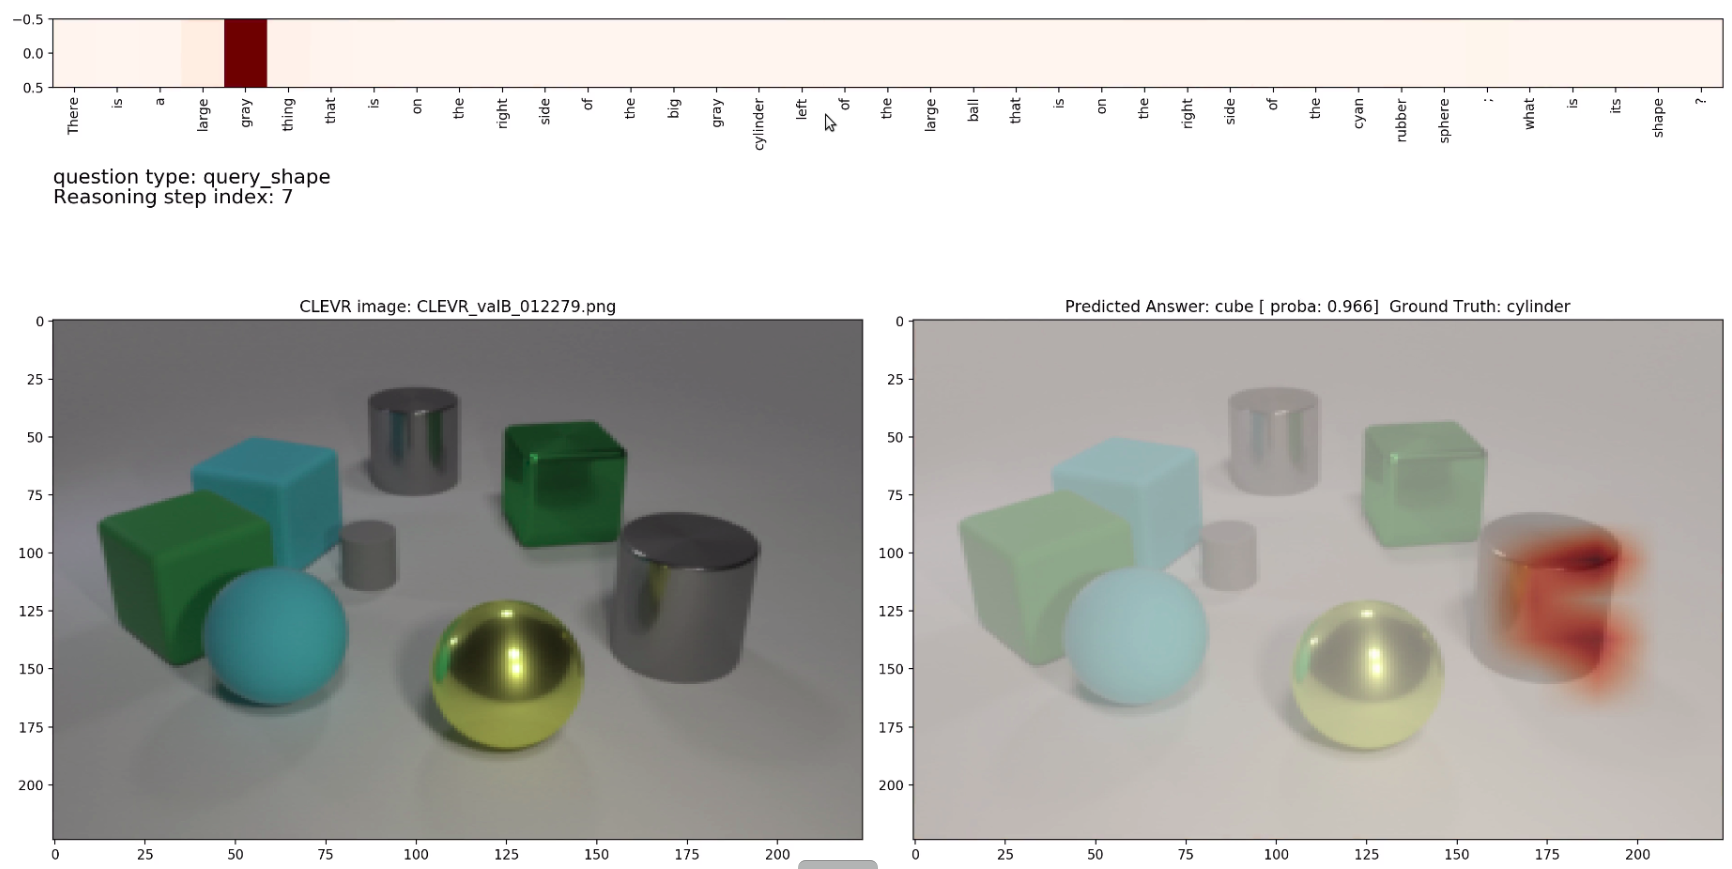
\includegraphics[width=\textwidth]{../img/fail_mac_cogent_b_shape.png}
	\caption{The question reads as: \textit{There is a large gray thing that is on the right side of the big gray cylinder left of the large ball that is on the right side if the cyan rubber sphere; what is its shape?}}
	\label{fig:fail_mac_shape}
\end{figure}

\begin{figure}[htbp]
	\centering
	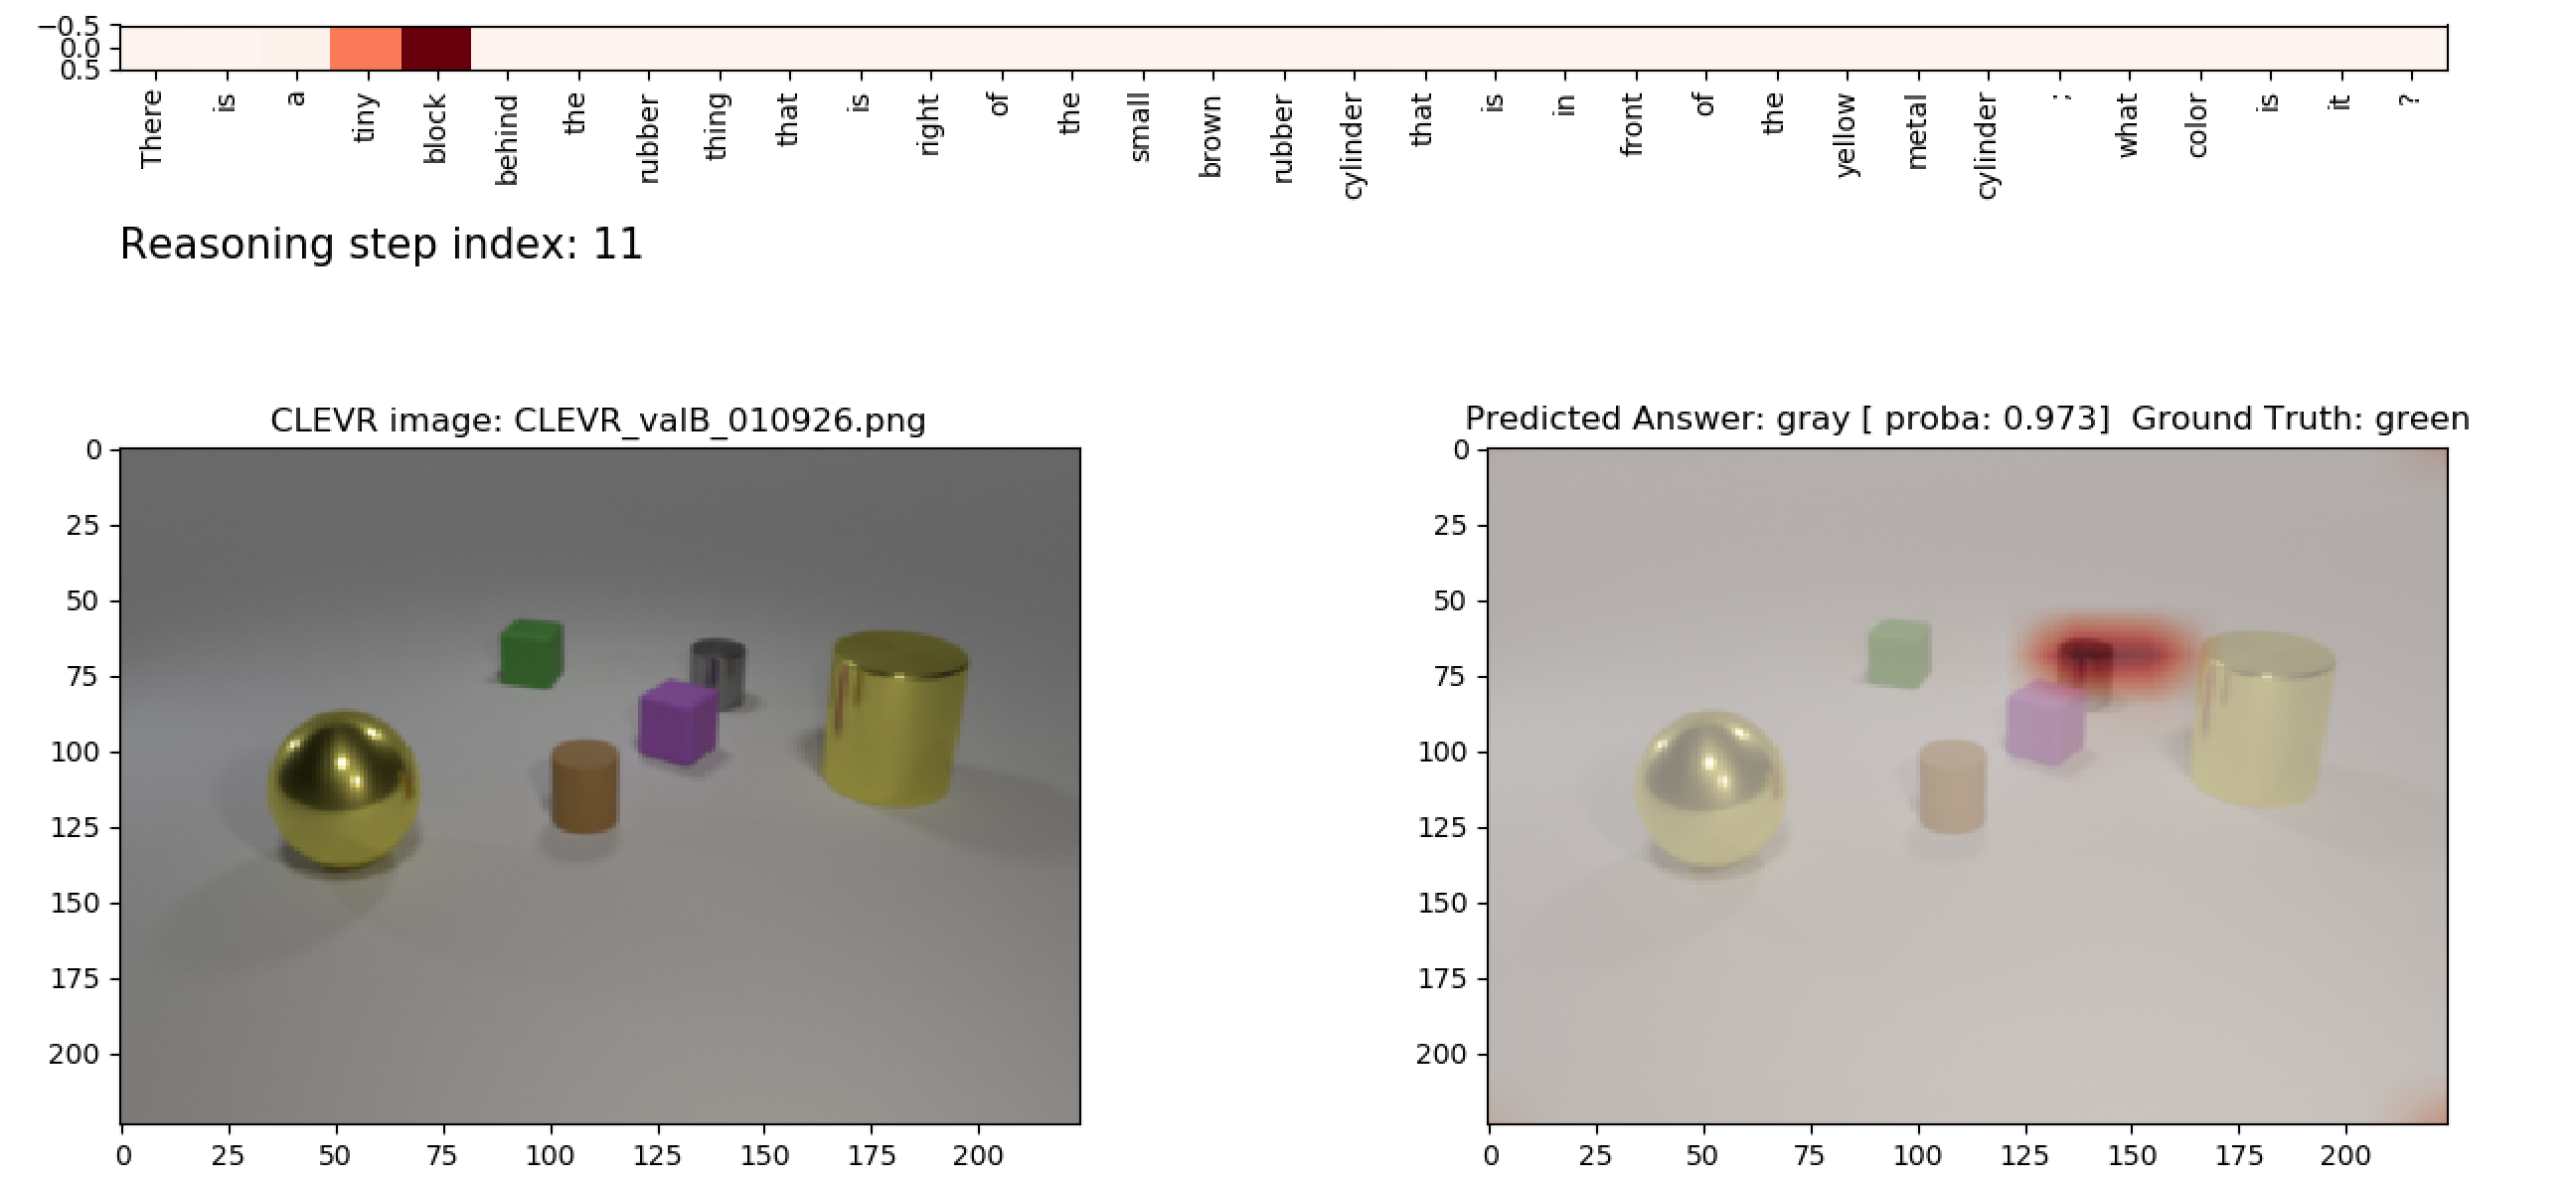
\includegraphics[width=\textwidth]{../img/fail_mac_cogent_b_color.png}
	\caption{The question reads as: \textit{There is a tiny block behind the rubber thing that is right if the small brown rubber cylinder that is in front of the yellow metal cylinder; what color is it?}}
	\label{fig:fail_mac_color}
\end{figure}

These examples indicate that MAC did not correctly separate the concept of shape from the concept of color, but have a better understanding of the colors (as it found the object of interest in \fig{fig:fail_mac_shape} by its color). This could come from that fact that the shape \textit{sphere} is associated with all possible colors in the dataset. 
